%!TeX spellcheck = fr-FR
\documentclass[10pt,fleqn]{article} % Default font size and left-justified equations
\usepackage[%
    pdftitle={SLCI : Transformée de Laplace},
    pdfauthor={Xavier Pessoles}]{hyperref}

\usepackage{import}
\usepackage{subcaption}
\subimport{../../../../style/}{preambule.tex}
%\fichetrue
\fichefalse
\proftrue
%\proffalse
%\tdtrue
\tdfalse
\courstrue
%\coursfalse
\subimport{../../../../style/}{new_style}
\subimport{../../../../style/}{macros_SII}
\subimport{../../../../style/}{preambule_trou.tex}

\usepackage{siunitx}
% -------------------------------------
% Déclaration des titres
% -------------------------------------

\def\discipline{Enseignement \\Technologique \\ Transversal}
\def\xxtete{Enseignement Technologique Transversal}

\def\classe{1 STI2D}
\def\xxnumpartie{Seq 3}
\def\xxpartie{Alimenter un système en énergie}

\def\xxnumchapitre{Séance 3}
\def\xxchapitre{\hspace{.12cm} Distribuer l'énergie}

\def\xxposongletx{2}
\def\xxposonglettext{1.45}
\def\xxposonglety{23}
\def\xxonglet{Seq. 3 -- Se. 3}

\def\xxactivite{Cours}
\def\xxauteur{\textsl{Geoffrey Vaquette}}

\def\xxcompetences{%
\textsl{%
\textbf{Savoirs et compétences :}
\begin{itemize}[label=\ding{112},font=\color{ocre}]
\item CO2.1	Identifier les flux et la forme de l'énergie, caractériser ses transformations et/ou modulations et estimer l'efficacité globale d'un système.
\end{itemize}
%
}}

\def\xxfigures{
\begin{center}
%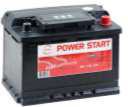
\includegraphics[width=2cm]{images/batterie.png} \\
%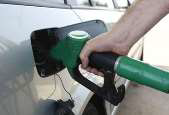
\includegraphics[width=2cm]{images/essence.png} \\
%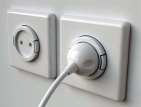
\includegraphics[width=2cm]{images/prise.png} \\
\end{center}
}%figues de la page de garde
\def\xxpied{%
La fonction alimenter/stocker \xxactivite%
}

%---------------------------------------------------------------------------

\renewcommand{\RemplirTrou}{false}
\begin{document}
\chapterimage{images/numerique}
\subimport{../../../../style/}{new_pagegarde}

\section{Généralités}
\subsection{La notion de variable}
\begin{definition}
  En informatique, les variables sont des symboles qui associent un nom (l'identifiant) à une valeur. Le nom d'une variable est \textbf{unique}.
\end{definition}


\subsection{Logique combinatoire}

\begin{definition}
  En informatique, la logique combinatoire désigne une logique dans laquelle l'état de la sortie d'un système ne dépend que de l'état des variables d'entrées. En particulier, l'état de la sortie ne dépend pas de l'état précédent de cette sortie.
\end{definition}

\begin{figure}[h]
  \centering
  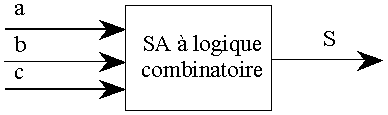
\includegraphics[width=.4\textwidth]{images/combinatoire}
  \caption{Logique combinatoire}
  \label{fig:combinatoire}
\end{figure}

\begin{exemple}
  Les phares d'un véhicule s'allument lorsque le conducteur actionne la commande. L'état des phares ne dépend donc que de l'état de la commande de phare.
\end{exemple}

\subsection{Logique séquentielle}

\begin{definition}
  En informatique, la logique séquentielle désigne une logique dans laquelle l'état de la sortie d'un système dépend de l'état des variables d'entrées ainsi que d'un état précédent du système.
\end{definition}

\begin{figure}[h]
  \centering
  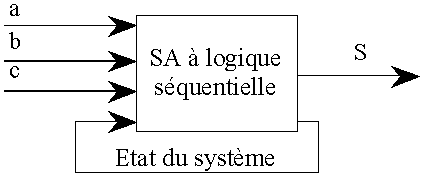
\includegraphics[width=.4\textwidth]{images/sequentiel}
  \caption{Logique séquentielle}
  \label{fig:combinatoire}
\end{figure}



\section{Différents types de signaux}
En automatique trois types de signaux sont utilisés principalement. Les signaux analogiques, numériques et tout ou rien.

\begin{figure}[ht]
  \begin{subfigure}{.33\textwidth}
    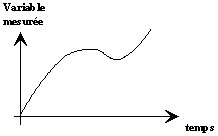
\includegraphics[width=\textwidth]{images/analogique}
    \caption{Signal analogique}
    \centering
    \label{fig:analogique}
  \end{subfigure}
  \begin{subfigure}{.33\textwidth}
    \centering
    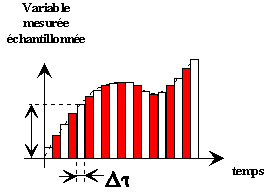
\includegraphics[width=\textwidth]{images/numerique}
    \caption{Signal numerique}
    \label{fig:numeique}
  \end{subfigure}
  \begin{subfigure}{.33\textwidth}
    \centering
    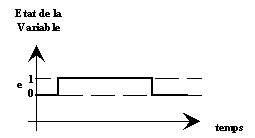
\includegraphics[width=\textwidth]{images/tor}
    \caption{Signal Tout ou Rien}
    \label{fig:tor}
  \end{subfigure}
\end{figure}

\subsection{Les signaux analogiques}
\begin{definition}
  Un signal analogique est un signal qui représente la variation continue d’une certaine grandeur (ex : température).
\end{definition}


\subsection{Les signaux numériques}
\begin{definition}
  Un signal numérique est un signal qui
représente la variation d’une grandeur par
succession de valeurs discrètes (ex : une
montre à affichage digital).
\end{definition}


\subsection{Les signaux Tout ou Rien (ToR)}
\begin{definition}
  Un signal tout ou rien est un signal qui représente l’état binaire (vrai, non
vrai) d’une variable d’un système (ex : un obstacle est présent (VRAI) ou absent (FAUX)).
\end{definition}


\section{La logique combinatoire}
\subsection{L'algèbre de Boole}
L'algèbre de Boole est la partie des mathématiques, de la logique et de l'électronique qui s'intéresse aux opérations et aux
fonctions sur les variables logiques. Le nom provient de
George Boole.
George Boole est le fondateur de la logique moderne.
L'algèbre de Boole est une algèbre permettant de traduire des signaux (tout ou rien) en expressions mathématiques en remplaçant
chaque signal élémentaire par des variables logiques et leur traitement par des fonctions logiques. L'algèbre de Boole permet de
résoudre des équations logiques afin de réaliser des fonctions sur des signaux numériques. Ces fonctions seront appelées fonctions
combinatoires

L'algèbre de Boole des fonctions logiques permet de modéliser des raisonnements logiques, en exprimant un « état » en fonction de conditions. un mathématicien britannique qui, durant le milieu du XIXe siècle, restructura complètement la
logique en un système formel. Plus spécifiquement, l'algèbre booléenne permet d'utiliser des techniques algébriques pour traiter les
expressions à deux valeurs de la
logique des propositions.
Aujourd'hui, l'algèbre de Boole trouve de nombreuses applications en informatique et dans la conception des circuits
électroniques.

\subsection{Etats des contacts et des récepteurs}
Un circuit électrique, électronique ou pneumatique, peut avoir 2 états logiques. Ces états peuvent prendre \textbf{les valeurs 1 ou 0}.
Ces états sont fonctions de l'état des composants en série dans le circuit.

\paragraph{Etat 0 :}
Les actionneurs tels que : moteurs, vérins sont à l'état 0 lorsqu'ils ne sont pas alimentés. Le circuit est alors ouvert. Pour un circuit
pneumatique ceci correspond à une absence de pression. Pour un circuit électrique cela correspond à une absence de différence de
potentiel entre les bornes du circuit.
Pour un contact ou un distributeur, c'est l’absence d'action physique intervenant sur un contact qui représente l'état 0.
\paragraph{État 1 :}
Les actionneurs sont à l'état 1 lorsqu'ils sont alimentés. Pour un circuit pneumatique ou hydraulique ceci correspond à une
pression d’air ou d’huile dans le circuit. Pour un circuit électrique cela correspond à une différence de potentiel entre les bornes du
circuit.
Pour un contact ou un distributeur ils sont actionnés, c’est à dire qu'une action physique est prise en compte.



\subsection{Table de vérité}
\begin{definition}
  Une table de vérité est la représentation de l’évolution du comportement d’un système automatisé en fonction des variations de
ses entrées. Chacune des variables est représentée sous une écriture binaire. Une table de vérité s'utilise principalement en \textbf{logique
combinatoire}.
\end{definition}

\begin{figure}
    \centering
  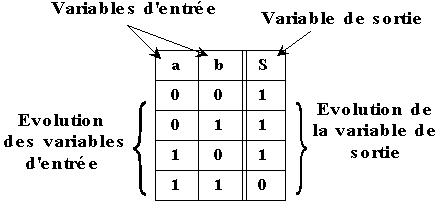
\includegraphics[width=.5\textwidth]{images/verite}
  \caption{Table de vérité d'un système}
  \label{fig:verite}
\end{figure}

\subsection{Logigramme}
\begin{definition}
  Un logigramme est un schéma représentant une succession de symboles logiques permettant d’obtenir par combinaison de
variables d’entrées la sortie recherchée. Attention, les fonctions logiques sont des opérateurs logiques et non des opérateurs
mathématiques. Le résultat obtenu sera un résultat logique et non un résultat mathématique.
\end{definition}
\begin{figure}[h]
  \centering
  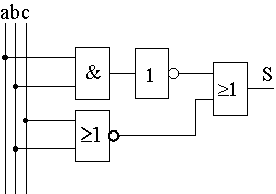
\includegraphics[width=.5\textwidth]{images/logigramme}
  \caption{Exemple de logigramme}
  \label{}
\end{figure}
\pagebreak
\subsection{Quelques fonctions logiques}
\subsubsection{Fonction OUI}
\begin{figure}[ht]
  \begin{subfigure}{.2\textwidth}
    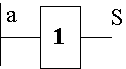
\includegraphics[width=\textwidth]{images/oui_symb}
    \caption{Symbole}
    \centering
  \end{subfigure}
  \begin{subfigure}{.4\textwidth}
    \centering
    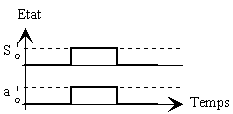
\includegraphics[width=\textwidth]{images/oui_chrono}
    \caption{Chonogramme}
  \end{subfigure}
  \begin{subfigure}{.33\textwidth}
    \centering
    \begin{tabular}{|c|c|}
      \hline
      \textbf{Entrée}& \textbf{Sortie} \\
      \hline
       & \\ \hline
       & \\ \hline
    \end{tabular}
    \caption{Table de vérité}
  \end{subfigure}
  \caption{Fonction OUI}
\end{figure}
\subsubsection{Fonction NON}
\begin{figure}[ht]
  \begin{subfigure}{.2\textwidth}
    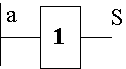
\includegraphics[width=\textwidth]{images/oui_symb}
    \caption{Symbole}
    \centering
  \end{subfigure}
  \begin{subfigure}{.4\textwidth}
    \centering
    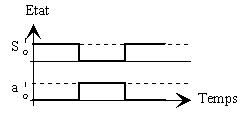
\includegraphics[width=\textwidth]{images/non_chrono}
    \caption{Chonogramme}
  \end{subfigure}
  \begin{subfigure}{.33\textwidth}
    \centering
    \begin{tabular}{|c|c|}
      \hline
      \textbf{Entrée}& \textbf{Sortie} \\
      \hline
       & \\ \hline
       & \\ \hline
    \end{tabular}
    \caption{Table de vérité}
  \end{subfigure}
  \caption{Fonction NON}
\end{figure}
\subsubsection{Fonction ET}
\begin{figure}[ht]
  \begin{subfigure}{.2\textwidth}
    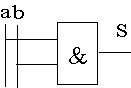
\includegraphics[width=\textwidth]{images/et_symb}
    \caption{Symbole}
    \centering
  \end{subfigure}
  \begin{subfigure}{.4\textwidth}
    \centering
    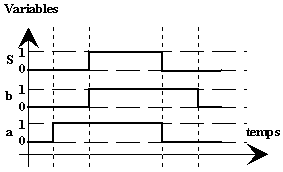
\includegraphics[width=\textwidth]{images/et_chrono}
    \caption{Chonogramme}
  \end{subfigure}
  \begin{subfigure}{.33\textwidth}
    \centering
    \begin{tabular}{|c|c|c|}
      \hline
      \textbf{a}&  \textbf{b}& \textbf{Sortie} \\
      \hline
       & & \\ \hline
       & & \\ \hline
       & & \\ \hline
       & & \\ \hline
    \end{tabular}
    \caption{Table de vérité}
  \end{subfigure}
  \caption{Fonction ET}
\end{figure}
\pagebreak
\subsubsection{Fonction OU}
\begin{figure}[ht]
  \begin{subfigure}{.2\textwidth}
    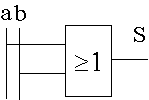
\includegraphics[width=\textwidth]{images/ou_symb}
    \caption{Symbole}
    \centering
  \end{subfigure}
  \begin{subfigure}{.4\textwidth}
    \centering
    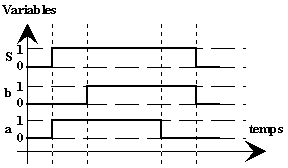
\includegraphics[width=\textwidth]{images/ou_chrono}
    \caption{Chonogramme}
  \end{subfigure}
  \begin{subfigure}{.33\textwidth}
    \centering
    \begin{tabular}{|c|c|c|}
      \hline
      \textbf{a}&  \textbf{b}& \textbf{Sortie} \\
      \hline
       & & \\ \hline
       & & \\ \hline
       & & \\ \hline
       & & \\ \hline
    \end{tabular}
    \caption{Table de vérité}
  \end{subfigure}
  \caption{Fonction OU}
\end{figure}
\subsubsection{Fonction NOR (NON OU)}
\begin{figure}[ht]
  \begin{subfigure}{.2\textwidth}
    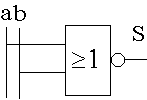
\includegraphics[width=\textwidth]{images/nor_symb}
    \caption{Symbole}
    \centering
  \end{subfigure}
  \begin{subfigure}{.4\textwidth}
    \centering
    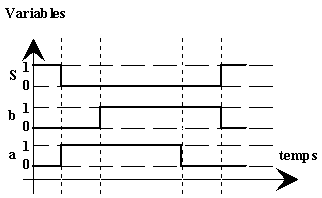
\includegraphics[width=\textwidth]{images/nor_chrono}
    \caption{Chonogramme}
  \end{subfigure}
  \begin{subfigure}{.33\textwidth}
    \centering
    \begin{tabular}{|c|c|c|}
      \hline
      \textbf{a}&  \textbf{b}& \textbf{Sortie} \\
      \hline
       & & \\ \hline
       & & \\ \hline
       & & \\ \hline
       & & \\ \hline
    \end{tabular}
    \caption{Table de vérité}
  \end{subfigure}
  \caption{Fonction NOR}
\end{figure}
\subsubsection{Fonction NAND (NON ET)}
\begin{figure}[ht]
  \begin{subfigure}{.2\textwidth}
    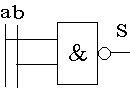
\includegraphics[width=\textwidth]{images/nand_symb}
    \caption{Symbole}
    \centering
  \end{subfigure}
  \begin{subfigure}{.4\textwidth}
    \centering
    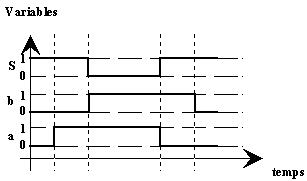
\includegraphics[width=\textwidth]{images/nand_chrono}
    \caption{Chonogramme}
  \end{subfigure}
  \begin{subfigure}{.33\textwidth}
    \centering
    \begin{tabular}{|c|c|c|}
      \hline
      \textbf{a}&  \textbf{b}& \textbf{Sortie} \\
      \hline
       & & \\ \hline
       & & \\ \hline
       & & \\ \hline
       & & \\ \hline
    \end{tabular}
    \caption{Table de vérité}
  \end{subfigure}
  \caption{Fonction NAND}
\end{figure}
\pagebreak
\subsubsection{Fonction OU EXCLUSIF}
\begin{figure}[ht]
  \begin{subfigure}{.2\textwidth}
    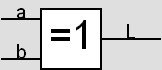
\includegraphics[width=\textwidth]{images/ouex_symb}
    \caption{Symbole}
    \centering
  \end{subfigure}
  \begin{subfigure}{.4\textwidth}
    \centering
    \vspace{3cm}
    \caption{Chonogramme}
  \end{subfigure}
  \begin{subfigure}{.33\textwidth}
    \centering
    \begin{tabular}{|c|c|c|}
      \hline
      \textbf{a}&  \textbf{b}& \textbf{Sortie} \\
      \hline
       & & \\ \hline
       & & \\ \hline
       & & \\ \hline
       & & \\ \hline
    \end{tabular}
    \caption{Table de vérité}
  \end{subfigure}
  \caption{Fonction OU EXCLUSIF}
\end{figure}

\subsection{Théorèmes de De Morgan}
\begin{theorem}
  Le complément d’un produit logique de variables est égal à la somme logique des compléments de variables.
  $$\overline{a \cdot b} = \overline{a} + \overline{b}$$
\end{theorem}

\begin{theorem}
  Le complément d’une somme logique de variables est égal au produit logique des compléments de variables.
  $$\overline{a+b} = \overline{a}\cdot\overline{b}$$
\end{theorem}

\end{document}
